\section{Reference module}
\label{sec:reference}
\begin{figure}[!h]
    \centering
    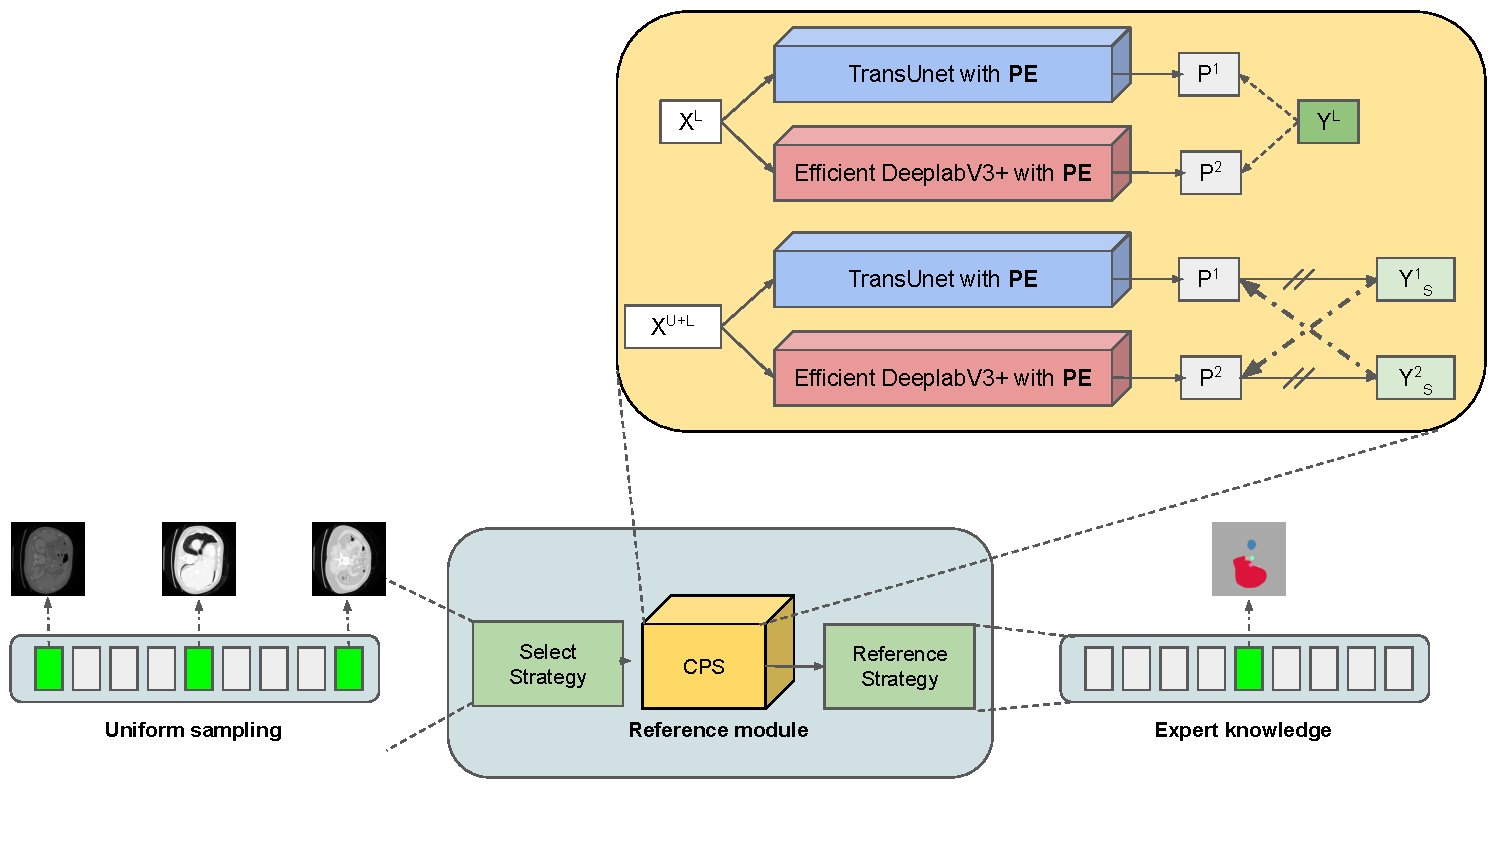
\includegraphics[width=\textwidth]{content/resources/new_images/reference.pdf}
    \caption{The reference module. The semi-supervised technique CPS is applied in both training and inference stage to enhance the precision of model prediction. Strategies are used to smartly choose slices that are informative for the next stage. }
    \label{fig:reference}
\end{figure}


This module is expected to provide a suggestion of a minimal amount of slices and predicted masks that might contain the most information describing the entire CT Volume. Fig \ref{fig:reference} describes the details of this module.

To utilize the enormous number of unlabeled data, we apply the recent semi-supervised method that performs effectively on several other datasets, which is called Cross Pseudo Supervision (CPS) \cite{chen2021semisupervised} (yellow cube in Fig. \ref{fig:reference}).
CPS enables the usage of unlabeled data by following the dual students technique, where two models are trained simultaneously on labeled data while generating pseudo data for their "peer" to learn. In the testing phase, two models predict the same image, and the result is aggregated by summing up.

We adopt two prominent state-of-the-arts 2D segmentation models with highly different learning paradigms for this CPS framework, which is TransUNet \cite{transunet21chen} and DeeplabV3+ \cite{dlv3p18chen}. While DeeplabV3+ traditionally focuses more on the local information, transformers model the long-range relation, so the cross training can help to learn a unified segmenter with these two properties at the same time. In short, we choose TransUNet and DeeplabV3+ due to their ability to compensate each other for better performance \cite{luo2021semisupervised}. 


\textbf{\textit{Positional Encoding}}. In order for the model to make use of the order of the sequence, we need to inject somne information about the position of the frames. For simplicity, we add an additional embedding layer to embed the relative position of the frame. Specifically, the embedded position index is concatenated with the hidden features before the final segmentation head. The relative position of $k^{th}$ frame of CT volume $i$ with length $T_i$ is calculated as:

\begin{align}
        PE(k) &= \frac{k}{T_i}
\end{align}

We attach this layer to both DeeplabV3+ and TransUnet. Since they follows conventional structure of segmentation models, which comprise of encoder and decoder phases, we manage to attach the layer in a similar way for both of them, as can be generally seen in Figure \ref{fig:pe_arch}

\begin{figure}[!h]
    \centering
    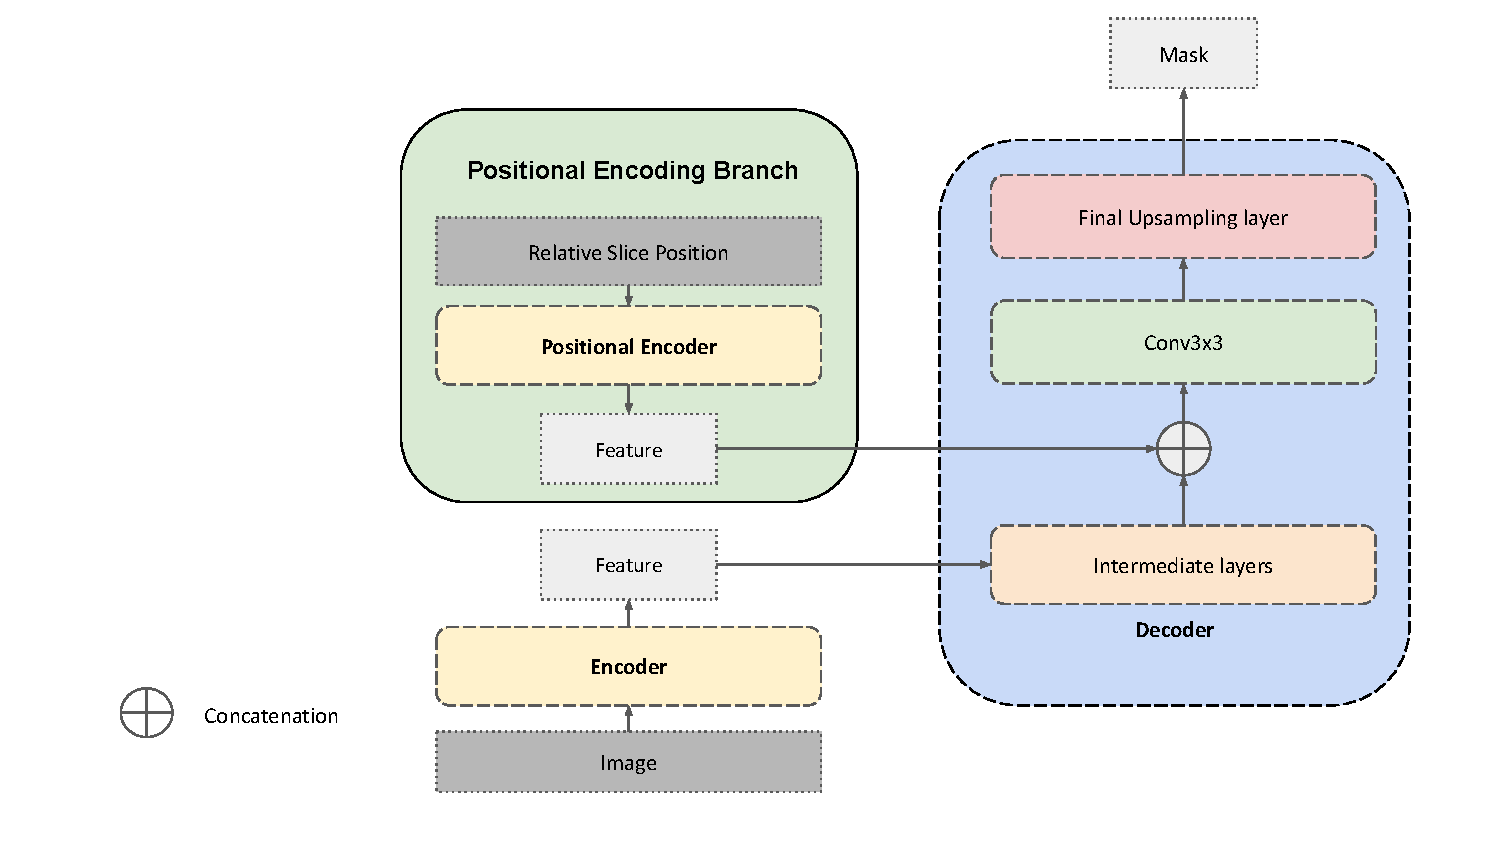
\includegraphics[width=\textwidth]{resources/new_images/pe.pdf}
    \caption{A general and simple way to attach a Positional Encoding branch into segmentation models . }
    \label{fig:pe_arch}
\end{figure}


In addition, we also propose a both logical and specialist-based strategy to choose which slices can be further used to boost the performance of the Propagation module. The goal of this action is to preserve only some of the most useful information for the refinement stage.

To elaborate on these strategies, prior to being put into the CPS module for prediction, a small number of slices are uniformly sampled from the processed CT volume. After CPS produces segmentation masks for these slices, another selection step is performed to pick only some of the masks that contain the organs having the largest areas.  